\chapter{Modele graficzne}

\section{Warunkowa niezależność cech}

Rozważmy \( x = [x_1, \dots, x_k] \) oraz daną wyjściową \( y \).

Mamy 
\begin{align*}
    p(x \given y)
        &= p(x_1, \dots, x_k \given y) \\
        &= p(x_1 \given y) \cdot p(x_2 \given y, x_1) \dots p(x_k \given y, x_1, \dots x_{k-1})
\end{align*}

Jeśli wszystkie cechy są binarne to aby opisać zachowanie takiego modelu potrzebujemy mieć aż 
\( 1 + 2 + 4 + \dots + 2^{k-1} = 2^k - 1 \) parametrów -- to dużo.

Jeśli założymy, że wszystkie te cechy są warunkowo niezależne to dostajemy
\[
    p(x \given y) = \prod_{i=1}^k p(x_i \given y)
\]
I tutaj wystarczy nam \( k \) parametrów.

\subsection{Przykład}

Załóżmy że mieszkamy w jakimś obszarze w którym mają miejsce trzęsienia ziemi i włamania. Dostaliśmy informację, że w domu włączył się alarm więc jedziemy do domu sprawdzić co się stało.
Podczas drogi powrotnej radiu powiedzieli, że miało miejsce lekkie trzęsienie ziemi. 

Zastanawiamy się teraz co faktycznie jest przyczyną alarmu i czy lepiej jest jechać się upewnić czy może wracać do roboty.

Mamy więc cztery binarne \textbf{zmienne losowe} (nie zdarzenia):
\begin{enumerate}
    \item E -- miało miejsce trzęsienie ziemi
    \item R -- radio podało informację o trzęsieniu
    \item B -- ktoś się do nas włamał
    \item A -- włączył się alarm
\end{enumerate}

Możemy rozpisać 
\[
    p(E, R, B, A) = p(E) \cdot p(B \given E) \cdot p(R \given E, B) \cdot p(A \given R, E, B)
\]
Mamy tutaj 15 parametrów, które musimy znać żeby znać pełen rozkład.

Jak się jednak dobrze zastanowimy to:
\begin{itemize}
    \item \( p(A \given R, E, B) = p(A \given E, B) \) -- to czy u nas działa alarm jest raczej niezależne od radia jeśli wiemy czy się do nas włamali i czy miało miejsce trzęsienie ziemii.
    
    \item \( p(R \given E, B) = p(R \given E) \) -- radio nie jest zainteresowane naszym domem.
    
    \item \( p(B \given E) = p(B) \) -- zakładamy że trzęsienie ziemi nie ma wpływu na włamania.
\end{itemize}

Powiedzmy że mamy jeszcze piątą zmienną \( N \), która mówi czy sąsiad do nas zadzwonił poinformować nas o alarmie.

Możemy zobrazować zależności za pomocą diagramu:

\begin{figure}[H]
    \centering
    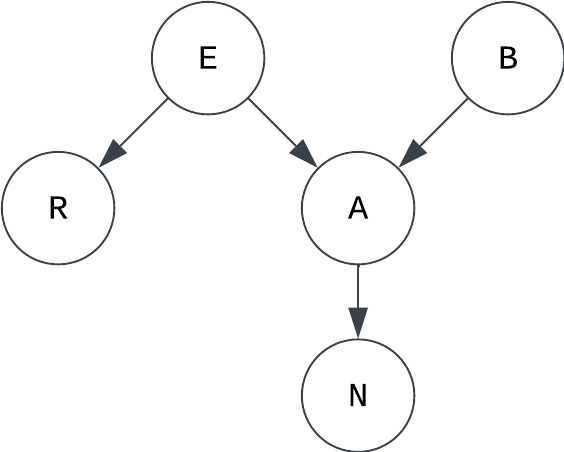
\includegraphics{chapters/graphical models/img/example.png}
    \caption{Model graficzny dla przykładu z trzęsieniem ziemi}
\end{figure}

\section{Model graficzny}

Model graficzny służy do wyrażenia zależności między zmiennymi losowymi za pomocą DAGu.

Bezpośrednie zależności między dwoma zmiennymi modelujemy jako krawędź skierowana od przyczyny do skutku.

Będziemy oznaczać \( X \perp Y \) jeśli te dwie zmienne są \textbf{niezależne}.

Jest kilka ciekawych struktur, które mogą wystąpić:
\begin{itemize}
    \item mediator
    \begin{figure}[H]
        \centering
        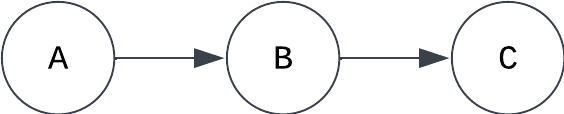
\includegraphics{chapters/graphical models/img/mediator.png}
        \caption{\( A \not \perp C \) ale \( A \perp C \given B \)}
    \end{figure}
    
    \item confounder
    
    \begin{figure}[H]
        \centering
        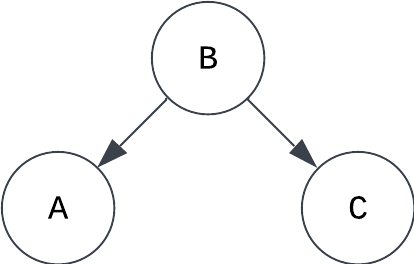
\includegraphics{chapters/graphical models/img/confounder.png}
        \caption{\( A \not \perp C \) ale \( A \perp C \given B \) }
    \end{figure}
    
    \item collider
    \begin{figure}[H]
        \centering
        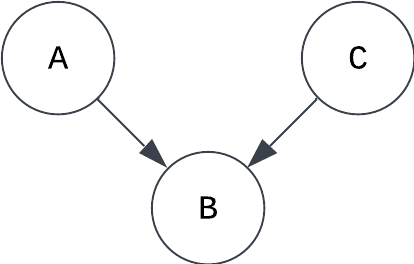
\includegraphics{chapters/graphical models/img/collider.png}
        \caption{\( A \perp C \) ale \( A \not \perp C \given B \) }
    \end{figure}
\end{itemize}

Aby sprawdzić czy dane dwie zmienne są od siebie zależne szukamy między nimi ścieżki zależności. Mediator i Confounder zamykają ścieżkę, natomiast Collider ją otwiera w momencie gdy warunkujemy się po zmiennej w danym węźle.

W naszym przykładzie z trzęsieniem ziemii mamy zatem \( E \perp B \), \( A \not \perp R \), \( B \perp R \) -- intuicyjne ma to sens, bo te rzeczy są od siebie naturalnie niezależnie.

Jeśli jednak wiemy czy alarm dzwoni czy nie to sytuacja się zmienia i mamy \( E \not \perp B, B \not \perp R \).  Jeśli wiemy że dzwoni alarm to sytuacja że w radiu nie ma informacji o trzęsieniu a do nas się nie włamują jest teraz bardzo mało prawdopodobna.

\begin{figure}[H]
    \centering
    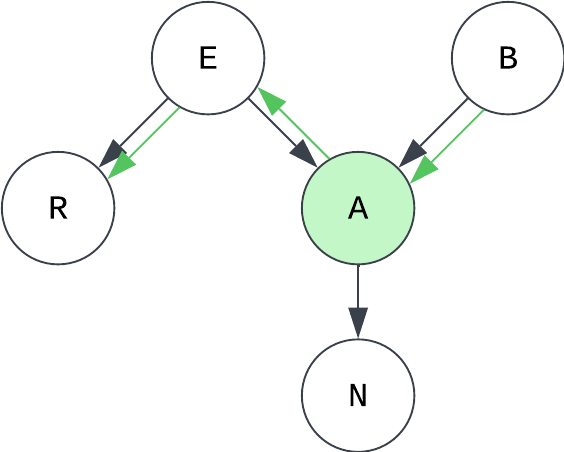
\includegraphics{chapters/graphical models/img/example-path.png}
    \caption{Ścieżka zależności \( B \not \perp R \given A \)}
\end{figure}